\chapter{Iteración 5: Diseño final de hardware} % (fold)
\label{cha:iteracion_5}

\section{Introducción} % (fold)
\label{it5:sec:introduccion}

Los distintos inconvenientes que surgieron en el desarrollo de las iteraciones 2, 3 y 4, nos obligo a analizar distintas alternativas para lograr cumplir por completo con los requerimientos 1.1 y 1.3. En iteraciones pasadas, se configuro el software y el hardware de la plataforma para poder tomar señales de hasta 2 contadores y hasta 4 señales en modo diferencial de 4 respectivos sensores. Esto no cumple con el numero mínimo de 4 contadores y 8 canales diferenciales. Si se duplicaran los recursos, llegaríamos a la cantidad requerida.

En esta iteración, intentamos aumentar las prestaciones de la plataforma duplicando los recursos de la placa construida en la iteración 3. Duplicando los recursos, alcanzaríamos los requerimientos de cantidad de contadores y canales de medición diferenciales.

% section introduccion (end)

\section{Requerimientos de la iteración} % (fold)
\label{it5:sec:requerimientos_de_la_iteracion}

A continuación, listamos los requerimientos de esta iteración.

\begin{itemize}
  \item Se deberían poder convertir a digital en modo canal único o diferencial, datos analógicos provenientes de hasta 8 sensores. [1.1]
  \item Se deberían poder contar eventos de hasta 4 señales externas. [1.3]
\end{itemize}

% section requerimientos_de_la_iteracion (end)

\section{Desarrollo} % (fold)
\label{it5:sec:desarrollo}

\subsection{Diseño Esquemático}
\label{it5:sub:diseño_esquematico2}

Para simplificar la explicación del diagrama, lo que haremos en esta sección es dividir el circuito entero en circuitos mas simples.

\subsubsection{Entradas Analógicas}
\label{it5:subs:entradas_analogicas2}

Los circuitos para las entradas analógicas son similares a los realizados en la iteración 3. Para cada una de las entradas se coloca un filtro pasa-bajo RC, como se muestra en la Figura \ref{fig:esquematicoFiltro}.

En la Figura \ref{fig:esquematicoFiltro2}, se muestran las entradas analógicas para un solo microcontrolador, siendo similar para el otro. En esta imagen, pueden verse las entradas analógicas con sus filtros, y además, dos pines PINHD\_AGND\_2. Estos pines son accesos a la masa digital para aquellos sensores que necesiten tener referencia a masa.

Del lado derecho del microcontrolador hay dos entradas denominadas VREF+ y VREF-, que sirven para manejar los niveles de tensión de referencia para el conversor.

\begin{figure}[h]
\centering
  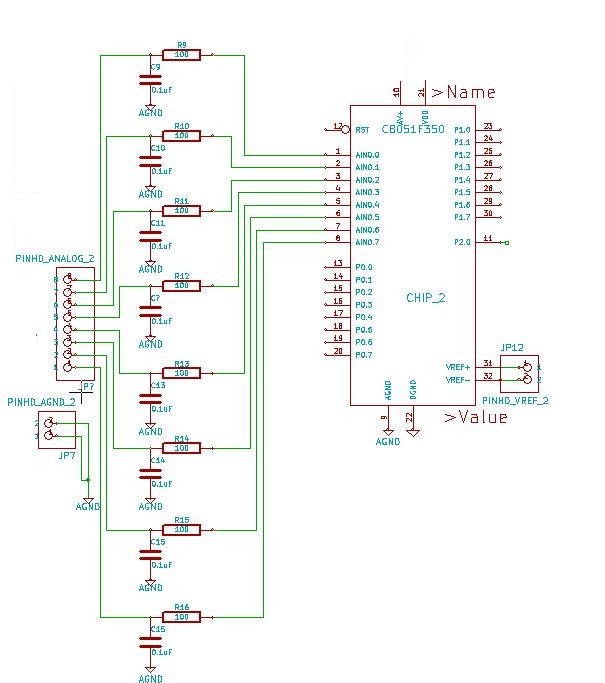
\includegraphics[width=1.10\textwidth, height = 9cm]{esquematicoFiltro2}
  \caption{Esquemático del Circuito Completo de entradas analógicas.}\label{fig:esquematicoFiltro2}
\end{figure}

% subsubsection entradas_analogicas2 (end)


\begin{figure}[h]
\centering
  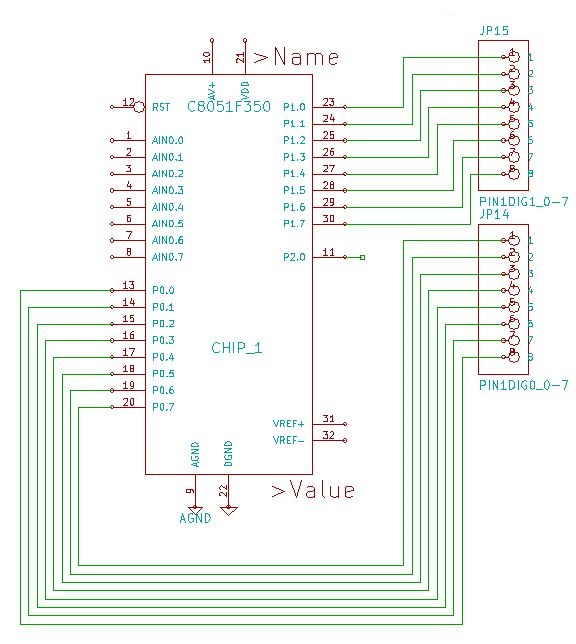
\includegraphics[width=1.0\textwidth, height = 10cm]{esquematicoDigital2}
  \caption{Esquemático del Circuito Completo de entradas/salidas digitales.}\label{fig:esquematicoDigital2}
\end{figure}


% subsubsection entradas_digitales (end)

\subsubsection{Circuito Salida Serial}
\label{it5:subs:salida_serial2}

Se reemplazo el circuito para la comunicación serial con adaptador RS-232 con un circuito simple de transmisor y receptor a nivel TTL. Esto tiene dos consecuencias importantes. La primera es que el sistema embebido que controle a la plataforma no podrá estar situado lejos de la misma ya que la aparición de errores en la comunicación tendrá una probabilidad mas alta. La segunda es que el tamaño de la plataforma se reduce, ya que no es necesario utilizar un adaptador RS-232, sino que solo se utilizan un par de pines para el transmisor Tx y el receptor Rx. Las salidas seriales se encuentran conectadas directamente en los pines de salidas digitales P0.4 (Tx) y P0.5(Rx).

% subsubsection salida_serial2 (end)

\subsubsection{Circuito para Debugger y Programación} % (fold)
\label{it5:subs:debugger_programacion2}

Por el momento, cada microcontrolador requiere que se programe por separado. Por una cuestión de simpleza, optamos por utilizar un mismo circuito de programación para ambos microcontroladores. Dentro del circuito, colocamos un selector que da la opción de elegir que microcontrolador se desea programar.

La Figura \ref{fig:esquematicoDebugger2} muestra el diagrama esquemático para el circuito de programación.

\begin{figure}  [H]
\centering
  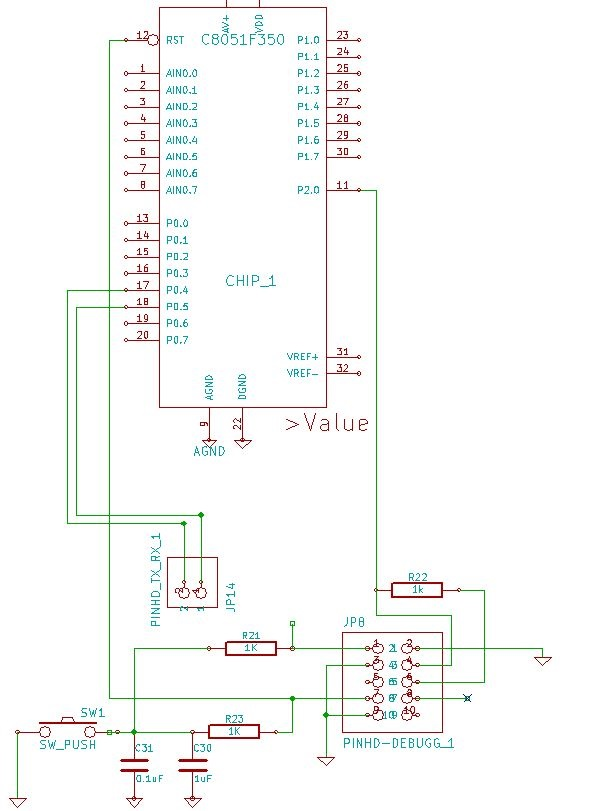
\includegraphics[width=1.0\textwidth, height = 8cm]{esquematicoDebugger2}
  \caption{Esquemático del Circuito para la programación de los microcontroladores de la placa.}\label{fig:esquematicoDebugger2}
\end{figure}


% subssubection debugger_programacion2 (end)

\subsubsection{Circuito de Alimentacion}
\label{subscircuito_de_alimentacion}

El circuito de alimentación es el mismo para ambos lados de la placa. Colocamos un jumper selector que cambia el origen de alimentación, pudiendo elegir entre el debugger o una fuente externa de 5 Volts.

Es posible, en caso que sea necesario, deshabilitar uno de los microcontroladores. De esta manera, se puede ahorrar energía cuando se este utilizando un microcontrolador, y el uso del otro no sea necesario. 

La Figura \ref{fig:esquematicoPotencia2} muestra el modelo esquemático del circuito de alimentación.

\begin{figure}[H] 
\centering
  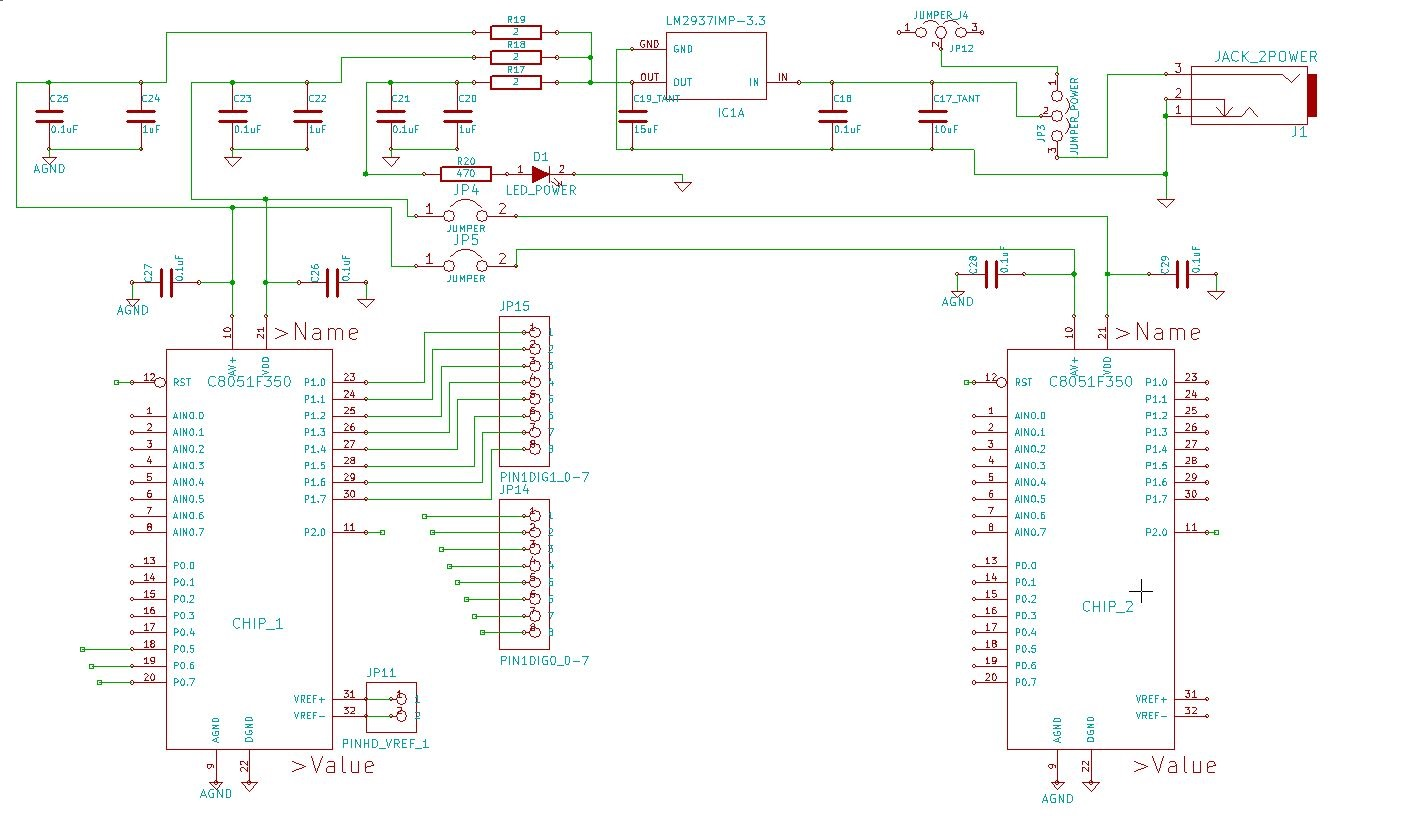
\includegraphics[width=1.0\textwidth, height = 10cm]{esquematicoPotencia2}
  \caption{Modelo esquemático del circuito de alimentación de la plataforma.}\label{fig:esquematicoPotencia2}
\end{figure}

%subsubsection circuito_potencia2 (end)

\subsubsection{Diagrama Esquemático Completo}
\label{subsubsection: esquematico_completo2}

En la Figura \ref{fig:esquematicoCompleto2} podemos ver como queda el esquemático entero con los dos microcontroladores y todos los circuitos que componen la placa.

\begin{figure}  
\centering
  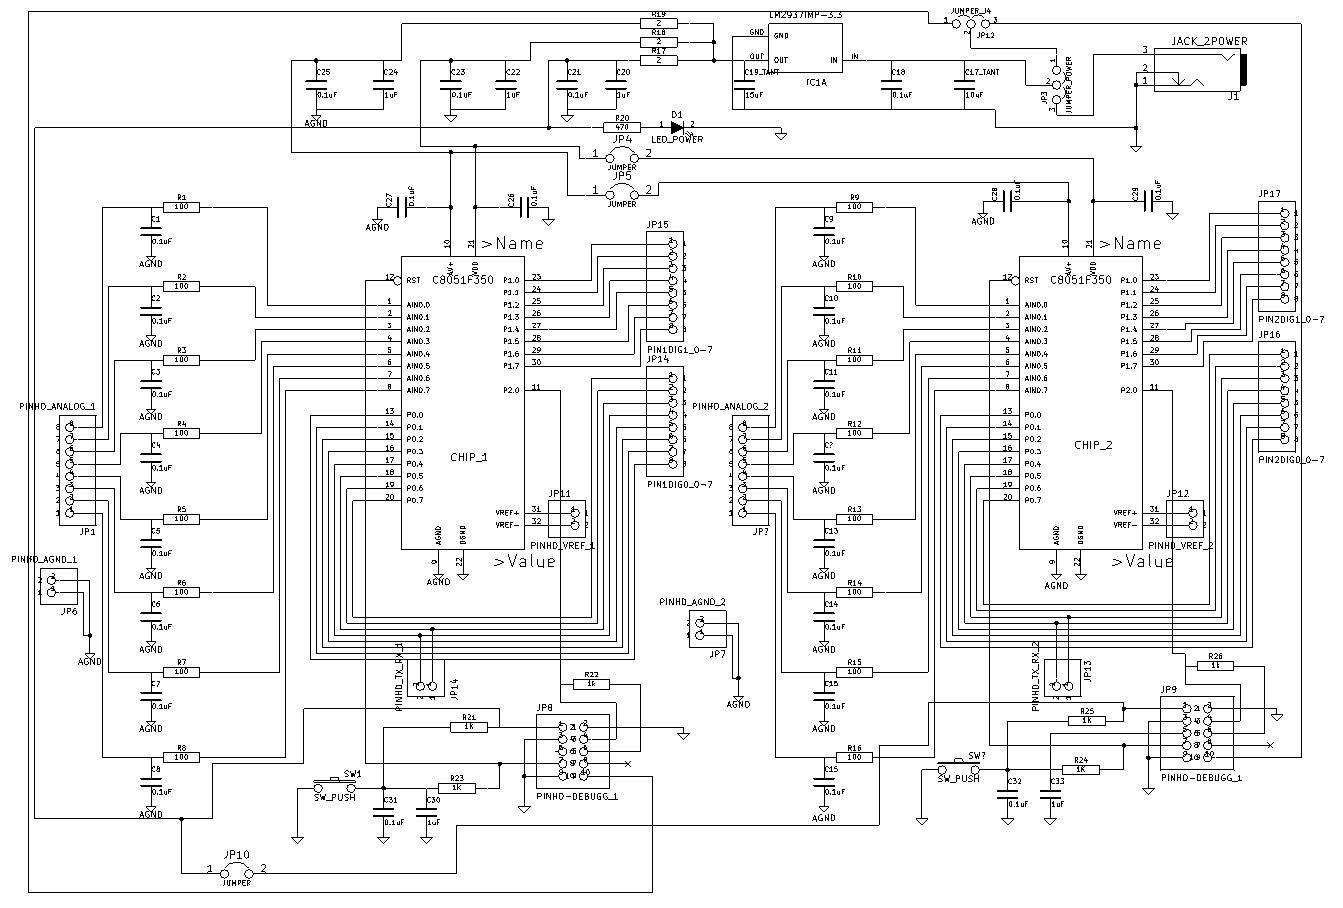
\includegraphics[width=1.10\textwidth, height = 12cm]{esquematicoCompleto2}
  \caption{Esquemático del Circuit completo de la Placa de desarrollo.}\label{fig:esquematicoCompleto2}
\end{figure}


% subsubsection esquematico_completo2 (end)

% subsection diseño_esquematico2 (end)

\subsection{Diseño de Plaqueta de Circuito Impreso (PCB)}
\label{ subsection: diseño_pcb2}

La figura \ref{fig:PCB2a} ilustra el diagrama en PCB de la capa superior o frontal de la placa. La figura  \ref{fig:PCB23Da} muestra esta misma capa, solo que utilizando un visualizador 3D.

Como esta nueva versión de la placa fue diseñada para ser doble capa, se mostrarán 2 figuras, una para la capa superior y otra para la capa inferior.

Existen dos masas distintas para cada lado de la placa: una masa analógica y otra digital. La masa analógica de un lado debería estar conectada con la masa analógica del otro lado, y así también para la masa digital. Para lograr esto, realizamos un hueco interconector, conectando las masas de cada placa.


\begin{figure}[H]
\centering
  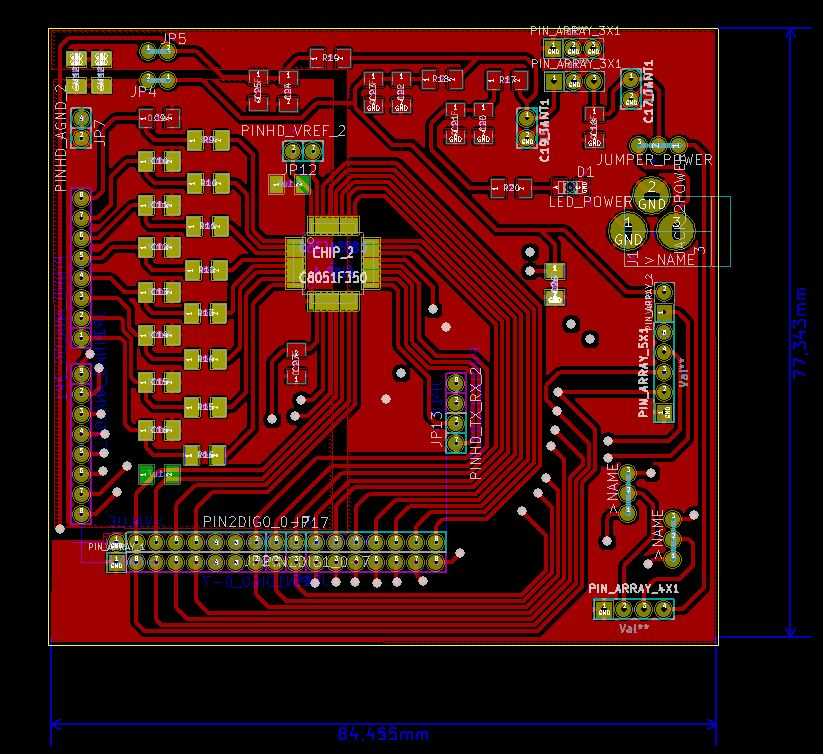
\includegraphics[width=1.0\textwidth, height = 8cm]{PCB2a}
  \caption{Diseño PCB de la capa frontal de la placa.}\label{fig:PCB2a}
\end{figure}

\begin{figure}  [H]
\centering
  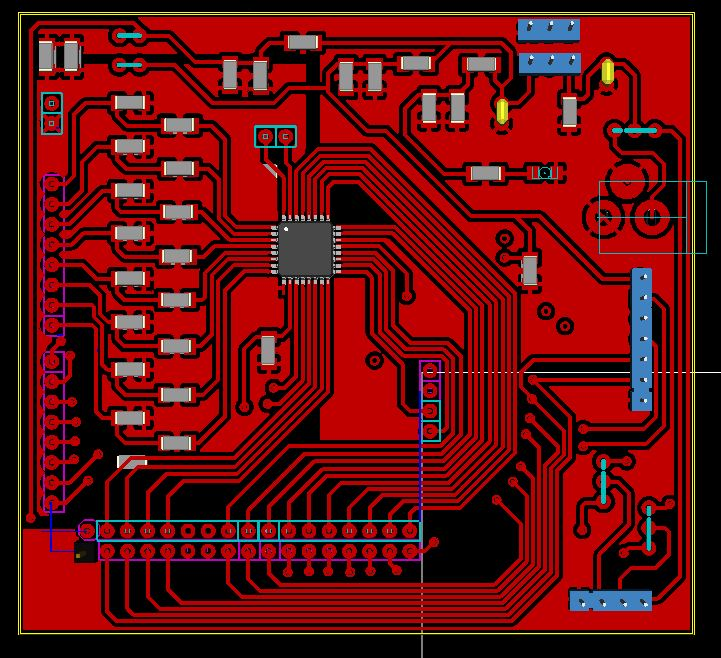
\includegraphics[width=1.0\textwidth, height = 8cm]{PCB23Da}
  \caption{Diseño PCB de la capa frontal de la placa en 3D.}\label{fig:PCB23Da}
\end{figure}

En la Figura \ref{fig:PCB2b} muestra el diagrama PCB de la capa inferior o posterior. La Figura \ref{fig:PCB23Db} muestra esta misma capa con el visualizador 3D.

\begin{figure}[h] 
\centering
  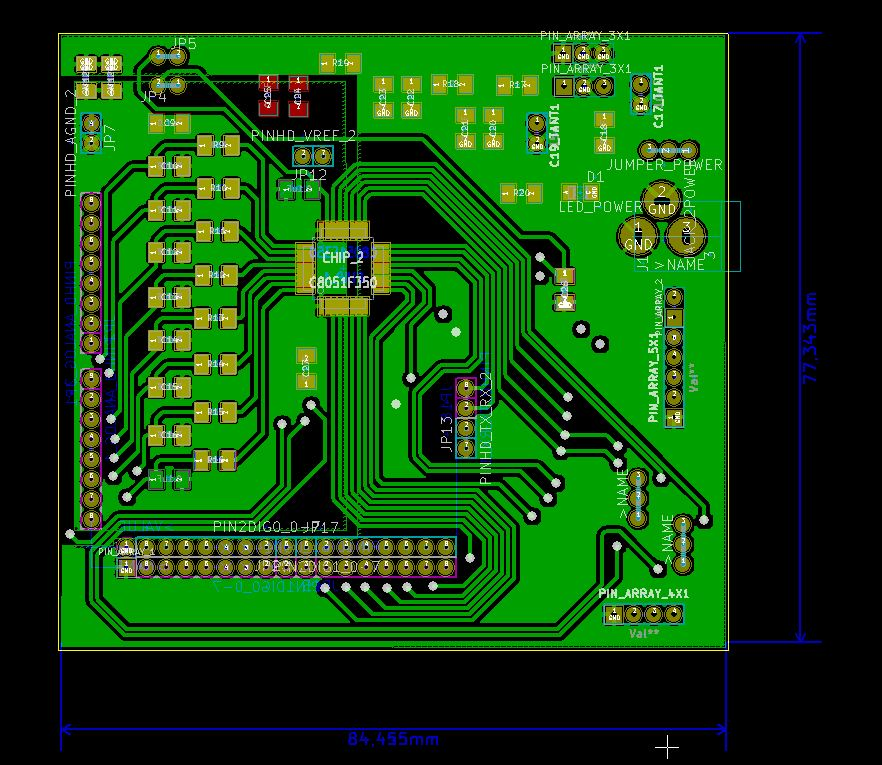
\includegraphics[width=1.0\textwidth, height = 8cm]{PCB2b}
  \caption{Diseño PCB de la capa posterior de la placa.}\label{fig:PCB2b}
\end{figure}

\begin{figure}  [h]
\centering
  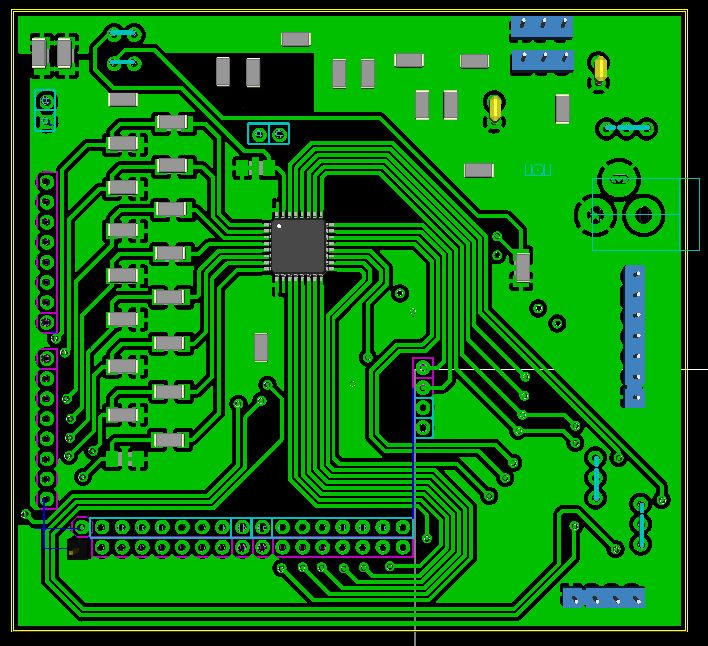
\includegraphics[width=1.0\textwidth, height = 8cm]{PCB23Db}
  \caption{Diseño PCB de la capa posterior de la placa en 3D.}\label{fig:PCB23Db}
\end{figure}


% subsection diseño_pcb2 (end)

\section{Pruebas} % (fold)
\label{it5:sec:pruebas}

\begin{table}[h]
\caption{Test de sistema 1: Correcto Diseño de PCB.}
\label{it4:tab:testsistema1}
\begin{tabular}{p{2cm} p{9cm}}
\multicolumn{2}{c}{\cellcolor[HTML]{68CBD0}{\color[HTML]{000000} Prueba de sistema}} \\
Prueba \#        & 1 \\
\hline
Nombre           & Correcto Diseño de PCB. \\
\hline
Requerimientos  &  1.1, 1.3, 1.6, 2.2 \\
\hline
Descripción      & Se verifica la existencia de errores en el diseño utilizando el ERC (perfom design rules check) que provee el software KiCad. \\
\hline
Pre-condiciones  & \tabitem Componentes colocados y pistas ruteadas. \\
                 & \tabitem Pads numerados con sus etiquetas.  \\
\hline
Post-condiciones & El resultado de ERC deberia ser cero. \\
\hline
Resultados       & No encontramos errores de diseño en el PCB. \\                                                                           
\end{tabular}
\end{table}

\begin{table}[h]
\caption{Test de sistema 2: Correcta impresión de la placa.}
\label{it4:tab:testsistema2}
\begin{tabular}{p{2cm} p{9cm}}
\multicolumn{2}{c}{\cellcolor[HTML]{68CBD0}{\color[HTML]{000000} Prueba de sistema}} \\
Prueba \#        & 2 \\
\hline
Nombre           & Correcta impresión de la placa.   \\

\hline
Requerimientos &    1.1, 1.3, 1.6, 2.2 \\
\hline
Descripción      & Corroboramos que todas las pistas y que todos los esquemas de perforado se hayan impreso correctamente. Luego, con un multímetro en modo continuidad, comprobamos que no existan cortocircuitos entre pistas y masa o entre pads y masa. \\
\hline
Pre-condiciones  & \tabitem Placa impresa. \\
                 & \tabitem Multímetro seteado en continuidad. \\
\hline
Post-condiciones & La placa debe tener las mismas pistas que aparecen en el diseño de PCB, y al medir con el multímetro nunca debe dar continuidad entre masa y pistas, o entre pads y pistas. \\
\hline
Resultados       & Todas las pistas se correspondían con el diseño de PCB.  \\                                                                                                                               
\end{tabular}
\end{table}

\begin{table}[h]
\centering
\caption{Test de sistema 3: Correcta soldadura de Componentes.}
\label{it4:tab:testsistema3}
\begin{tabular}{p{2cm} p{9cm}}
\multicolumn{2}{c}{\cellcolor[HTML]{68CBD0}{\color[HTML]{000000} Prueba de sistema}} \\
Prueba \#        & 3 \\
\hline
Nombre           & Correcta soldadura de Componentes. \\
\hline
Requerimientos &    1.1, 1.3, 1.6, 2.2   \\
\hline
Descripción      & Se utiliza el multímetro en modo continuidad para poder comprobar si existen cortocircuitos y verificar si todos los componentes están bien interconectados. \\
\hline
Pre-condiciones  & \tabitem Placa impresa. \\
                 & \tabitem Pistas impresas correctamente. \\
                 & \tabitem Componentes soldados. \\
                 & \tabitem Multímetro seteado en continuidad. \\
\hline
Post-condiciones &  No debería haber cortocircuitos, y la interconexión entre los distintos componentes debería corresponderse con el diseño de PCB. \\ 
\hline
Resultados       & Encontramos cortocircuitos luego de soldar los componentes. Fue necesario des-soldar algunos componentes y volverlos a colocar para solucionar el problema. \\
\end{tabular}
\end{table}

\begin{table}[h]
\centering
\caption{Test de sistema 4: Correcta Comunicación Con SiliconLabs Debugger.}
\label{it4:tab:testsistema4}
\begin{tabular}{p{2cm} p{9cm}}
\multicolumn{2}{c}{\cellcolor[HTML]{68CBD0}{\color[HTML]{000000} Prueba de sistema}} \\
Prueba \#        & 4 \\
\hline
Nombre           & Correcta Comunicación Con SiliconLabs Debugger. \\
\hline
Requerimientos &  \tabitem Se debería poder conectar el debugger del microcontrolador a la placa para poder programarlo. \\
\hline
Descripción      & Se utilizo el cable USB con el debugger de SiliconLabs para conectar la placa a la PC. \\
\hline
Pre-condiciones  & 3.2 \\
\hline
Post-condiciones &  Al abrir la IDE y accionar el botón de "Connect", el programa debe reconocer el tipo de microcontrolador al que esta conectado. \\ 
\hline
Resultados       &  Conectamos la placa al ordenador e intentamos conectarla con el microcontrolador a través de la IDE. El resultado fue el esperado, el microcontrolador estaba exitosamente conectado al ordenador. \\
\end{tabular}
\end{table}

\begin{table}[h]
\centering
\caption{Test de sistema 5: Correcta programación del microcontrolador.}
\label{it4:tab:testsistema5}
\begin{tabular}{p{2cm} p{9cm}}
\multicolumn{2}{c}{\cellcolor[HTML]{68CBD0}{\color[HTML]{000000} Prueba de sistema}} \\
Prueba \#        & 4 \\
\hline
Nombre           & Correcta programación del microcontrolador. \\
\hline
Requerimientos &  3.2 \\                                   
\hline
Descripción      & Se utilizo el cable USB con el debugger de SiliconLabs para conectar la placa a la PC y descargarle un programa .hex al microcontrolador. \\
\hline
Pre-condiciones  & \tabitem Placa impresa. \\
                 & \tabitem Pistas impresas correctamente. \\
                 & \tabitem Componentes soldados. \\
                 & \tabitem IDE SiliconLabs instalada en la PC. \\
                 & \tabitem IDE SiliconLabs reconociendo el C8051f352. \\
\hline
Post-condiciones &  Al abrir la IDE y apretar el botón de "Connect" el programa debe reconocer el tipo de microcontrolador al que esta conectado y luego a través de la misma IDE o del "Flash Programing Utilitys" cargarle un programa .hex al c8051f352. \\ 
\hline
Resultados       &  Conectamos la placa a la PC y desde el software "Flash Programing Utilitys" se pudo cargar un programa a los microcontroladores soldados en la placa. \\                                                                                                  
\end{tabular}
\end{table}

\begin{table}[h]
\centering
\caption{Test de sistema 6: Correcto funcionamiento de las entradas analógicas y salidas digitales.}
\label{it4:tab:testsistema6}
\begin{tabular}{p{2cm} p{9cm}}
\multicolumn{2}{c}{\cellcolor[HTML]{68CBD0}{\color[HTML]{000000} Prueba de sistema}} \\
Prueba \#        & 4 \\
\hline
Nombre           & Correcto funcionamiento de las entradas analógicas y salidas digitales. \\                      

\hline
Requerimientos &    1.1 \\
\hline
Descripción      & Se cargo un programa de prueba a ambos microcontroladores. Utilizando una fuente de tensión, introducimos distintos valores de tensión en dos canales en modo único, uno de cada microcontrolador. Luego, utilizamos ambas plataformas para convertir los datos a digital y verificar que la telemetría medida concuerde con el nivel de tensión generado. \\
\hline
Pre-condiciones  & \tabitem Componentes conectados y soldados correctamente en la placa. \\
                 & \tabitem IDE SiliconLabs iniciado y corriendo en un ordenador. \\
                 & \tabitem Microcontrolador conectado y reconocido por el software de Silicon Labs. \\
                 & \tabitem Programa de prueba correctamente cargado en el C8051f352. \\
                 & \tabitem Fuente de Tensión externa conectada a las entradas analógicas con referencia en masa analógica. \\
\hline
Post-condiciones &  Al apretar el botón de "Go" en el programa "Flash Programing Utilitys", se inicia el programa. Configurando los canales conectados e iniciando las conversiones continuas, deberían comenzar a aparecer las mediciones realizadas sobre los canales. Las mediciones deberían corresponderse con los valores de tensión establecidos en las fuentes conectadas. \\
\hline
Resultados       &  Cargamos el programa en el microcontrolador, y con todas las pre-condiciones cumplidas hicimos correr el programa. Los valores de tensión medidos se correspondían con los establecidos en la fuente. \\                                                                                                            
\end{tabular}
\end{table}


% section pruebas (end)

\section{Conclusiones} % (fold)
\label{it5:sec:conclusiones}


Al final de esta iteración, obtuvimos una plataforma con dos microcontroladores y el doble de recursos que la diseñada anteriormente. Esto permite con los requisitos de cantidad de contadores y cantidad de canales de conversión diferencial, ligados a los requerimientos 1.1 y 1.3.
Aun así, todavía queda trabajo por hacer. Aunque los recursos estén duplicados, es necesario vincular ambas plataformas, para que trabajen en conjunto y no en paralelo. De esta forma, pasa a ser una única plataforma con el doble de recursos, y no dos plataformas en un único espacio físico.

En esta iteración, llegamos a unir dos plataformas en un único lugar físico, pero sin correlación su funcionamiento.

En la Figura \ref{fig:impresionplaca2_a} y \ref{fig:impresionplaca2_b} podemos ver como quedo la placa final, tanto de la capa superior como de la inferior. Se acomodaron los componentes de manera tal que los pines y módulos que se pueden utilizar para conectar alguna interfaz/cable, queden en la misma capa.

\begin{figure}  
\centering
  \includegraphics[width=1.10\textwidth, height = 12cm]{impresionplaca2_a}
  \caption{Circuito de Hardware final ya impreso.}\label{fig:impresionplaca2_a}
\end{figure}

\begin{figure}  
\centering
  \includegraphics[width=1.10\textwidth, height = 12cm]{impresionplaca2_b}
  \caption{Circuito de Hardware final ya impreso.}\label{fig:impresionplaca2_b}
\end{figure}



% section resultados (end)

% chapter iteracion_5 (end)